\documentclass{article}%
\usepackage[T1]{fontenc}%
\usepackage[utf8]{inputenc}%
\usepackage{lmodern}%
\usepackage{textcomp}%
\usepackage{lastpage}%
\usepackage[head=40pt,margin=0.5in,bottom=0.6in]{geometry}%
\usepackage{graphicx}%
%
\title{\textbf{Escasez de gas detona dos protestas en la carretera Panamericana}}%
\author{Diario El Universal}%
\date{05/10/2018}%
%
\begin{document}%
\normalsize%
\maketitle%
\textbf{URL: }%
http://www.eluniversal.com/caracas/22426/escasez{-}de{-}gas{-}detona{-}dos{-}protestas{-}en{-}la{-}carretera{-}panamericana\newline%
%
\textbf{Periodico: }%
EU, %
ID: %
22426, %
Seccion: %
caracas\newline%
%
\textbf{Palabras Claves: }%
NO\_TIENE\newline%
%
\textbf{Derecho: }%
2.8, %
Otros Derechos: %
, %
Sub Derechos: %
2.8.1\newline%
%
\textbf{EP: }%
SI\newline%
\newline%
%
\textbf{\textit{Con bombonas en la vía pública, compradores se atravesaron en la avenida Pedro Russo Ferrer de Los Teques, obstaculizando el paso en ambos sentido y afectando en flujo vehicular}}%
\newline%
\newline%
%
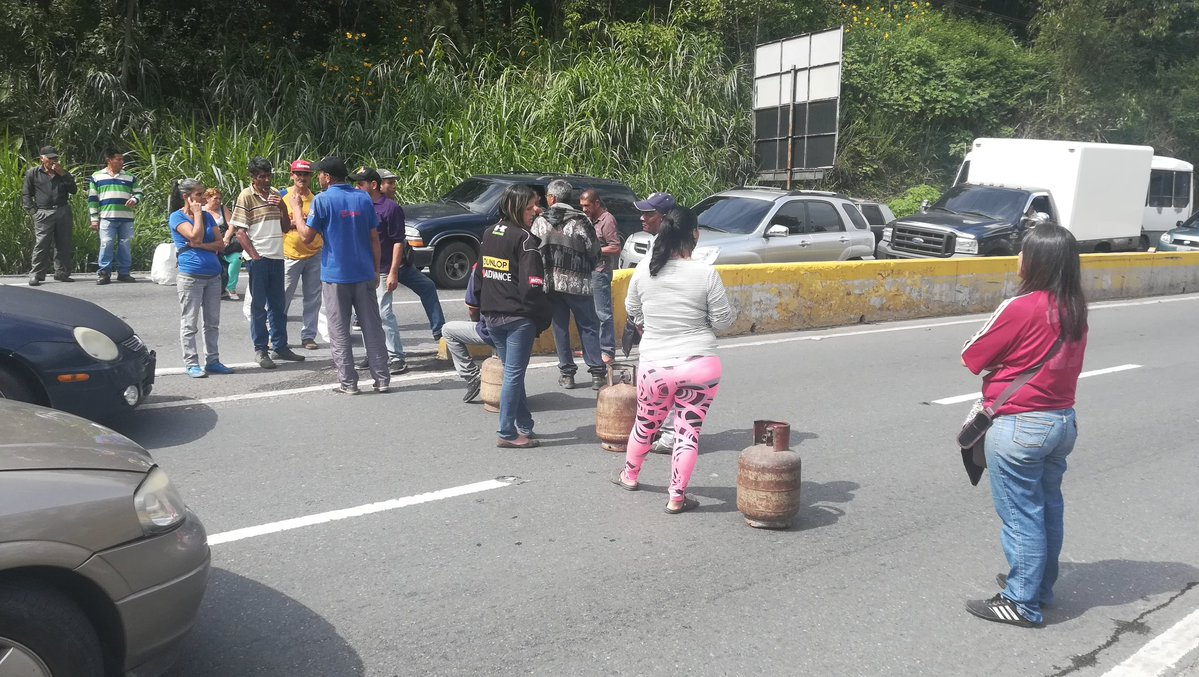
\includegraphics[width=300px]{236.jpg}%
\newline%
%
Los Teques.  Camiones fuera de servicio por falta de repuestos y un sistema de distribución no óptimo serían las principales causas de la escasez de gas en los Altos Mirandinos, problemática que detonó dos protestas en menos de una semana en la carretera Panamericana, siendo la más reciente la mañana de este viernes.%
\newline%
%
Con bombonas en la vía pública, compradores se atravesaron en la avenida Pedro Russo Ferrer de Los Teques, obstaculizando el paso en ambos sentido y afectando en flujo vehicular en el distribuidor Los Cerritos en la carretera Panamericana aproximadamente a las 10:00 a.m.%
\newline%
%
“Estamos desde las 2 de la madrugada en las afueras del llenadero de Pdva Gas Comunal en Los Cerritos  esperando poder llenar nuestra bombona y resulta que después de pasar frío y exponernos al peligro de ser atracados nos dicen que no alcanza para todo el mundo. Es una falta de respeto constante”, refirió Graciela Sulbarán, quien ante la precariedad en el servicio, se ha visto obligada a cocinar a leña en las afueras de su hogar en el barrio El Nacional de la capital mirandina.%
\newline%
%
{-}{-}Ya ni quienes tienen cocina eléctrica se salvan porque con las recientes lluvias los apagones están a la orden del día, así que más gente necesita del gas y el servicio cada vez es más deficiente. Ya perdí la cuenta del tiempo que llevo sin ver un camión de gas en mi barrio. El otro tema son los precios, porque una cosa es lo que marca y otra muy distinta es lo que uno paga. La última vez que vendieron en la comunidad eso parecía una subasta porque la bombona se la llevaba quien pagara más.%
\newline%
%
La acción fue replicada el martes 2 de octubre, cuando los compradores trancaron en el mismo punto por la misma causa. “Las colas cada vez son más largas y sin embargo uno hace el sacrificio porque es una necesidad, pero se burlan de nosotros al no tener capacidad de atender más que, si acaso, al 30 \% de las personas que acuden”, denunció Carmen Quijada, habitante de la avenida Bicentenario de Los Teques.%
\newline%
%
{-}{-}Es contradictorio porque vivo al lado de la funeraria José Gregorio Hernández y veo desde la ventana de mi apartamento a escasos metros, al lado, cuando llega el camión a surtirlos mientras a nosotros nos ignoran deliberadamente. Como no tengo carro y no me permiten montarme en el autobús con la bombona por obvias medidas de seguridad, me toca pagar el sobreprecio de la bombona más transporte. Lo que vivimos es un caos diario y no parece que fuera a mejorar en el corto ni mediano plazo. Todo empeora.%
\newline%
%
\end{document}